% Options for packages loaded elsewhere
\PassOptionsToPackage{unicode}{hyperref}
\PassOptionsToPackage{hyphens}{url}
\PassOptionsToPackage{dvipsnames,svgnames,x11names}{xcolor}
%
\documentclass[
]{jds}

\usepackage{amsmath,amssymb}
\usepackage{iftex}
\ifPDFTeX
  \usepackage[T1]{fontenc}
  \usepackage[utf8]{inputenc}
  \usepackage{textcomp} % provide euro and other symbols
\else % if luatex or xetex
  \usepackage{unicode-math}
  \defaultfontfeatures{Scale=MatchLowercase}
  \defaultfontfeatures[\rmfamily]{Ligatures=TeX,Scale=1}
\fi
\usepackage{lmodern}
\ifPDFTeX\else  
    % xetex/luatex font selection
\fi
% Use upquote if available, for straight quotes in verbatim environments
\IfFileExists{upquote.sty}{\usepackage{upquote}}{}
\IfFileExists{microtype.sty}{% use microtype if available
  \usepackage[]{microtype}
  \UseMicrotypeSet[protrusion]{basicmath} % disable protrusion for tt fonts
}{}
\makeatletter
\@ifundefined{KOMAClassName}{% if non-KOMA class
  \IfFileExists{parskip.sty}{%
    \usepackage{parskip}
  }{% else
    \setlength{\parindent}{0pt}
    \setlength{\parskip}{6pt plus 2pt minus 1pt}}
}{% if KOMA class
  \KOMAoptions{parskip=half}}
\makeatother
\usepackage{xcolor}
\setlength{\emergencystretch}{3em} % prevent overfull lines
\setcounter{secnumdepth}{-\maxdimen} % remove section numbering
% Make \paragraph and \subparagraph free-standing
\ifx\paragraph\undefined\else
  \let\oldparagraph\paragraph
  \renewcommand{\paragraph}[1]{\oldparagraph{#1}\mbox{}}
\fi
\ifx\subparagraph\undefined\else
  \let\oldsubparagraph\subparagraph
  \renewcommand{\subparagraph}[1]{\oldsubparagraph{#1}\mbox{}}
\fi


\providecommand{\tightlist}{%
  \setlength{\itemsep}{0pt}\setlength{\parskip}{0pt}}\usepackage{longtable,booktabs,array}
\usepackage{calc} % for calculating minipage widths
% Correct order of tables after \paragraph or \subparagraph
\usepackage{etoolbox}
\makeatletter
\patchcmd\longtable{\par}{\if@noskipsec\mbox{}\fi\par}{}{}
\makeatother
% Allow footnotes in longtable head/foot
\IfFileExists{footnotehyper.sty}{\usepackage{footnotehyper}}{\usepackage{footnote}}
\makesavenoteenv{longtable}
\usepackage{graphicx}
\makeatletter
\def\maxwidth{\ifdim\Gin@nat@width>\linewidth\linewidth\else\Gin@nat@width\fi}
\def\maxheight{\ifdim\Gin@nat@height>\textheight\textheight\else\Gin@nat@height\fi}
\makeatother
% Scale images if necessary, so that they will not overflow the page
% margins by default, and it is still possible to overwrite the defaults
% using explicit options in \includegraphics[width, height, ...]{}
\setkeys{Gin}{width=\maxwidth,height=\maxheight,keepaspectratio}
% Set default figure placement to htbp
\makeatletter
\def\fps@figure{htbp}
\makeatother

\makeatletter
\@ifpackageloaded{caption}{}{\usepackage{caption}}
\AtBeginDocument{%
\ifdefined\contentsname
  \renewcommand*\contentsname{Table of contents}
\else
  \newcommand\contentsname{Table of contents}
\fi
\ifdefined\listfigurename
  \renewcommand*\listfigurename{List of Figures}
\else
  \newcommand\listfigurename{List of Figures}
\fi
\ifdefined\listtablename
  \renewcommand*\listtablename{List of Tables}
\else
  \newcommand\listtablename{List of Tables}
\fi
\ifdefined\figurename
  \renewcommand*\figurename{Figure}
\else
  \newcommand\figurename{Figure}
\fi
\ifdefined\tablename
  \renewcommand*\tablename{Table}
\else
  \newcommand\tablename{Table}
\fi
}
\@ifpackageloaded{float}{}{\usepackage{float}}
\floatstyle{ruled}
\@ifundefined{c@chapter}{\newfloat{codelisting}{h}{lop}}{\newfloat{codelisting}{h}{lop}[chapter]}
\floatname{codelisting}{Listing}
\newcommand*\listoflistings{\listof{codelisting}{List of Listings}}
\makeatother
\makeatletter
\makeatother
\makeatletter
\@ifpackageloaded{caption}{}{\usepackage{caption}}
\@ifpackageloaded{subcaption}{}{\usepackage{subcaption}}
\makeatother
\ifLuaTeX
  \usepackage{selnolig}  % disable illegal ligatures
\fi
\usepackage{bookmark}

\IfFileExists{xurl.sty}{\usepackage{xurl}}{} % add URL line breaks if available
\urlstyle{same} % disable monospaced font for URLs
\hypersetup{
  pdftitle={My wonderful paper},
  colorlinks=true,
  linkcolor={blue},
  filecolor={Maroon},
  citecolor={Blue},
  urlcolor={Blue},
  pdfcreator={LaTeX via pandoc}}

\title{My wonderful paper}
\author{}
\date{}

\begin{document}
\maketitle
\begin{abstract}
This is the abstract
\end{abstract}

\section{Introduction}\label{introduction}

In this paper, a concept called analysis plan is proposed to describe
the logical structure of a data analysis. An analysis plan is a set of
analysis steps plus their expected outcomes. It is a formal
representation of the analysis process and can be used to guide the
analysis process, to communicate and compare the analysis process to
others, and to evaluate the analysis process. The concept of analysis
plan is illustrated with examples and the implications of the concept
for data analysis practice is discussed.

The analysis plan described in this paper should be differentiated from
the pre-specifies analysis plan document often used in biostatistics to
specifies the hypothesis, data collection mechanism, statistical
procedures etc of randomized experiments.

\section{Analysis plan}\label{analysis-plan}

describe/ define what analysis plan is

analysis plan and outcome plan

analysis plan as unit tests to divide the ``result universe'', which
allows us to answer questions like:

\begin{itemize}
\tightlist
\item
  how would the results change if the value of a unit test change
\item
  whether our outcome expectation aligns with the plan expectation,
  meaning whether ``it is possible for the combination of plan
  expectations to produce the outcome expectation''
\end{itemize}

\section{Examples}\label{examples}

\subsection{A toy example}\label{a-toy-example}

\subsection{Linear regression}\label{linear-regression}

Consider a linear regression model to study the effect of PM10 on
mortality (provide context of using PM10 to study mortality). From the
literature, analysts may expect a significant PM10 coefficient in the
linear model from the literature. This is the outcome expectation:
p-value of PM10 coefficient is less than 0.05. There are multiple
factors that can affect the outcome expectation of this analysis, for
example, 1) sample size, 2) model specification, and 3) correlation
structure between variables. Temperature is often an important
confounder to consider in such study (add reference).

To construct the result universe, we can simulate datasets with
different configerations of the above factors. Here, sample sizes of 50,
100, 500, and 1000 are considered. Two model specifications are
included: 1) linear model with PM10 as the only covariate
(\(\text{mortality} \sim \text{PM10}\)), 2) linear model with PM10 and
temperature as covariates
(\(\text{mortality} \sim \text{PM10} + \text{temp}\). A grid-based
approach is used to simulate correlation structure. Reasonable ranges of
correlation between the three variables are

\begin{align*}
\text{cor}(\text{mortality}, \text{PM10}) &\in [-0.01, 0] \\ 
\text{cor}(\text{mortality}, \text{temperature}) &\in [-0.6, -0.2] \\ \text{cor}(\text{PM10}, \text{temperature}) &\in [0.2, 0.6] 
\end{align*}

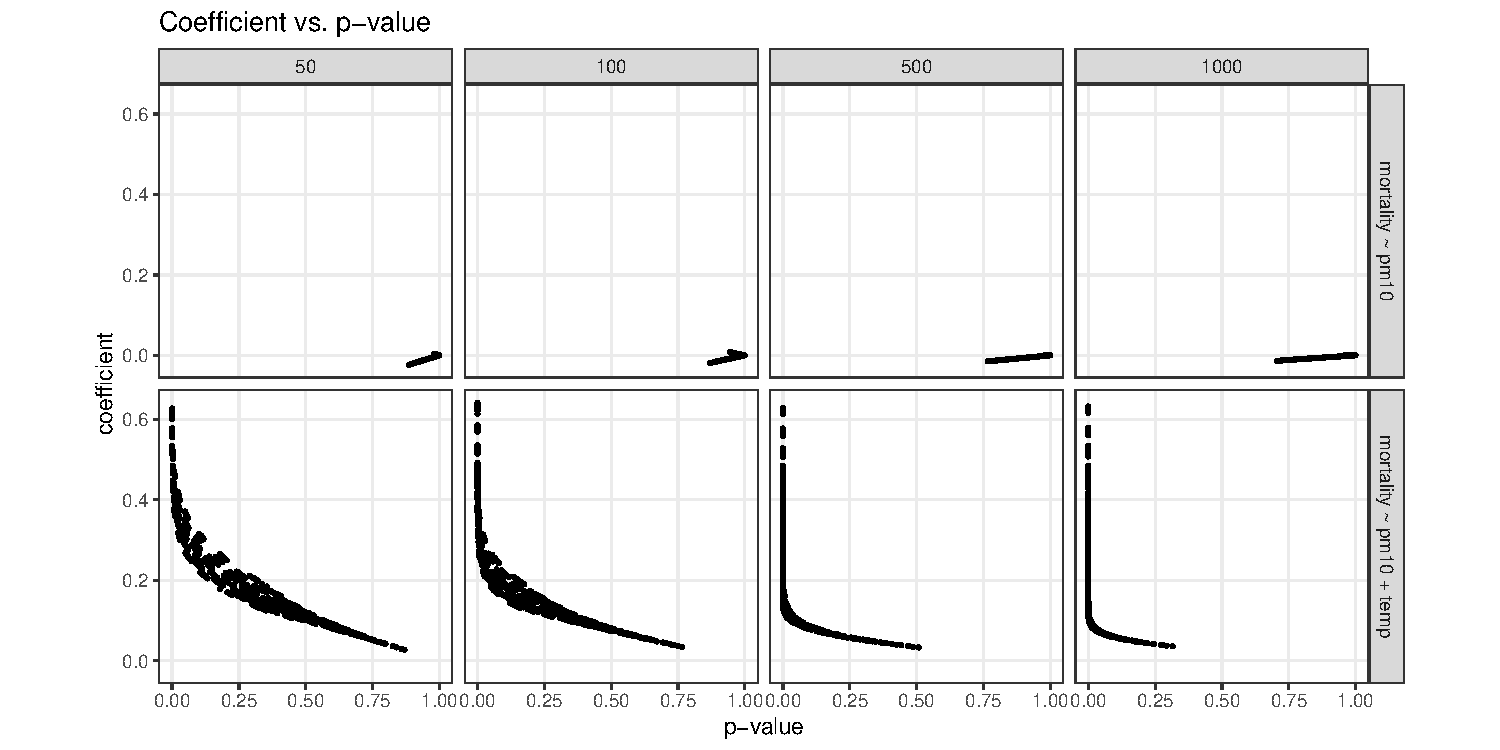
\includegraphics{index_files/figure-pdf/unnamed-chunk-2-1.pdf}

\phantomsection\label{cell-fig-result-universe}
\begin{figure}[H]

\centering{

\captionsetup{labelsep=none}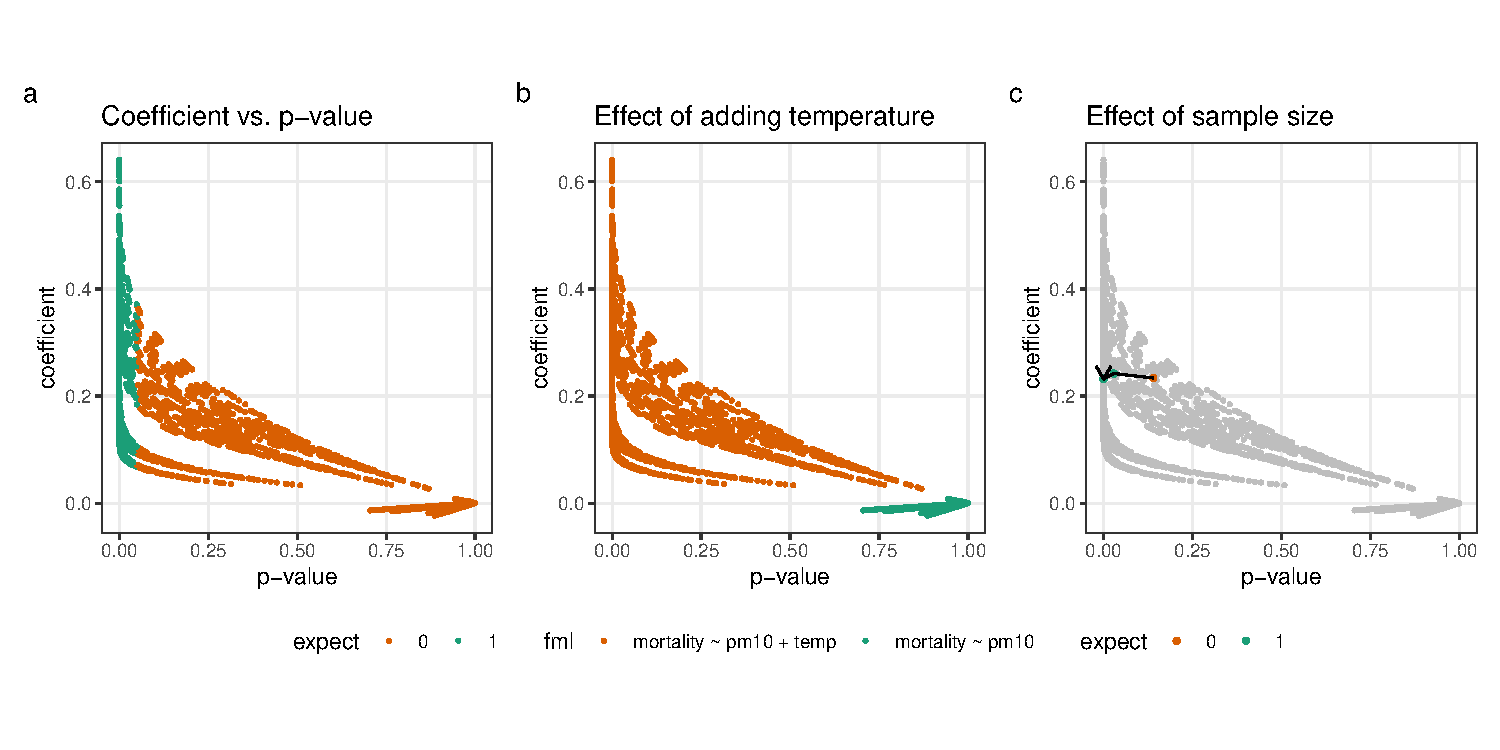
\includegraphics{index_files/figure-pdf/fig-result-universe-1.pdf}

}

\caption{\label{fig-result-universe}}

\end{figure}%

Figure~\ref{fig-result-universe} shows that result universe of the
linear regression model with a) colored by whether the p-value of PM10
is significant (less than 0.05), b) highlighting the effect of adding
temperature to the model for a fixed correlation structure, and c)
highlighting the effect of increasing sample size.



\end{document}
